\documentclass{standalone}
\usepackage{tikz}
\usepackage{amssymb}

\begin{document}
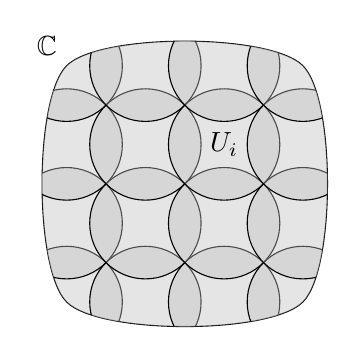
\begin{tikzpicture}
	\draw (0,3) node[anchor=south east]{$ \mathbb{C} $};
	\draw plot[smooth cycle] coordinates{(0,0) (3,0) (3,3) (0,3)};
	\begin{scope}
		\clip plot[smooth cycle] coordinates{(0,0) (3,0) (3,3) (0,3)};
		\foreach \a in {0,1,...,3}{
				\foreach \b in {0,1,...,3}{
						\filldraw[fill = gray!50, fill opacity = 0.4] (\a, \b) circle
						({sqrt(2)/2});
					}
			};
		\draw (2,2) node{$ U_i $};
	\end{scope}
\end{tikzpicture}
\end{document}
